\documentclass{article}
\usepackage{graphicx} % Required for inserting images

\title{DSCI 372M Homework 1}
\author{Steven Sanchez}
\date{January 2026}

\begin{document}

\maketitle

\section*{Question 1}
\subsection*{Part (a):}
\subsubsection*{$ \hat{y} =  w_0 + w_1 x_1 + w_2 x_2, Error = \hat{y} - y $}

$ \hat{y_1} =  0 + 0(1) + 0(1) = 0 $, Error = 0 - (-0.8) = 0.8

$ \hat{y_2} =  0 + 0(-1) + 0(-2) = 0 $, Error = 0 - (0.1) = -0.1

$ \hat{y_3} =  0 + 0(2) + 0(-1) = 0 $, Error = 0 - (-5.0) = 5.0


\subsubsection*{Mean Squared Error: $ \frac{1}{3} [(0.8)^2 + (-0.1)^2 + (5.0)^2] = 8.55$ }

$ w_0: \frac{2}{3} (0.8 - 0.1 + 5.0) = 3.8$ , $w_0 = 0 - 0.05(3.8) = -0.19 $

$ w_1: \frac{2}{3} (0.8(1) - 0.1(-1) + 5.0(2)) = 7.26$, $ w_1 = 0 - 0.05(7.26) = -0.363$

$ w_2: \frac{2}{3} (0.8(1) - 0.1(-2) + 5.0(-1)) = -2.66 $ $w_2 = 0 - 0.05(-2.66) = 0.133$

\subsubsection*{New weights: $w_0, w_1, w_2 = -0.19, -0.363, 0.133$}

\begin{figure}
    \centering
    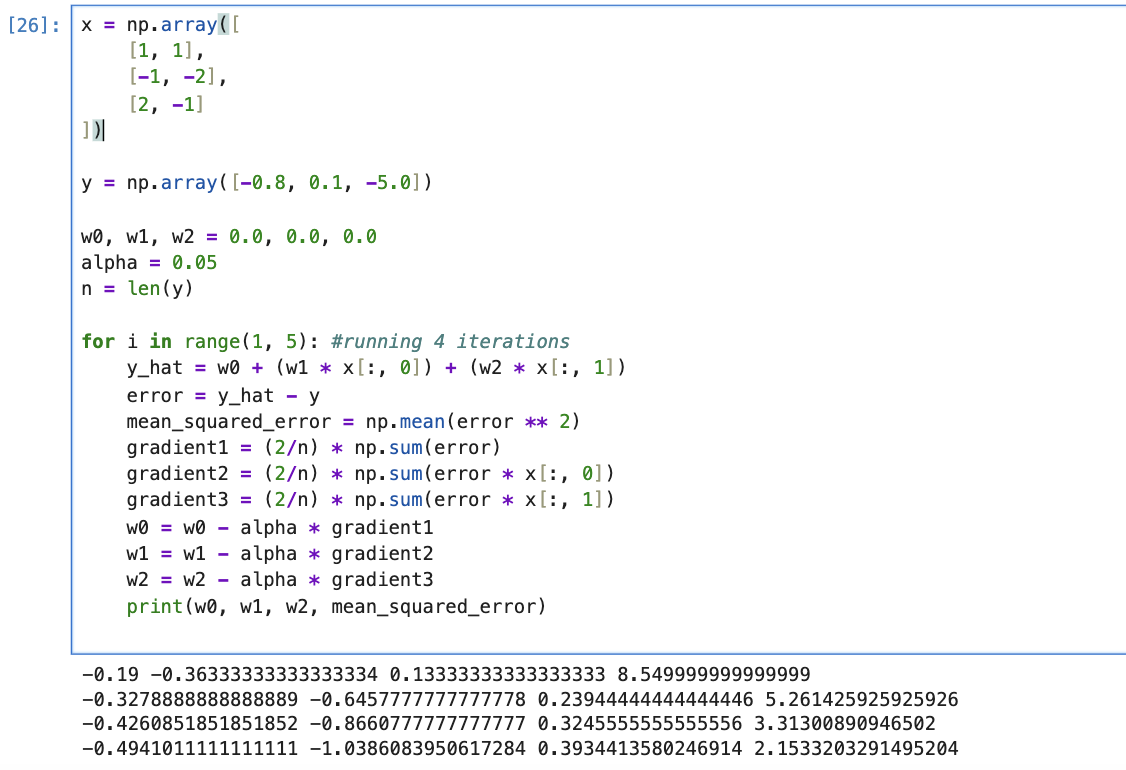
\includegraphics[width=0.5\linewidth]{image.png}
    \label{fig:placeholder}
\end{figure}


\begin{center}
\begin{tabular}{|c|c|c|c|c|}
\hline
Iteration & $w_0$ & $w_1$ & $w_2$ & MSE \\
\hline
1 & -0.19 & -0.36 & 0.13 & 8.55 \\
2 & -0.36 & -0.65 & 0.24 & 5.26 \\
3 & -0.43 & -0.87 & 0.32 & 3.31 \\
4 & -0.49 & -1.04 & 0.39 & 2.15 \\
\hline
\end{tabular}
\end{center}

The code above shows the iteration for the next 3, but we showed the step by step process for the first one so we can visually see what is happening.

\subsection*{Part (b):}
For this, we learned back in MA342: w = $(X^T X)^{-1}X^TY$

Here, we have our matrices: 

X =
\begin{tabular}{|c|c|c|}
\hline
1 & 1 & 1 \\
1 & -1 & -2 \\
1 & 2 & -1 \\
\hline
\end{tabular}
and Y = 
\begin{tabular}{|c|}
\hline
 -0.8 \\
0.1 \\
-5.0 \\
\hline
\end{tabular}
where $ X^T $ is the transpose of X (basically flipping the rows and columns).

$(\begin{tabular}{|c|c|c|}
\hline
1 & 1 & 1 \\
1 & -1 & 2 \\
1 & -2 & -1 \\
\hline
\end{tabular}
*
\begin{tabular}{|c|c|c|}
\hline
1 & 1 & 1 \\
1 & -1 & -2 \\
1 & 2 & -1 \\
\hline
\end{tabular})^{-1}$
*
\begin{tabular}{|c|c|c|}
\hline
1 & 1 & 1 \\
1 & -1 & 2 \\
1 & -2 & -1 \\
\hline
\end{tabular}
\begin{tabular}{|c|}
\hline
 -0.8 \\
0.1 \\
-5.0 \\
\hline
\end{tabular}
= 
\begin{tabular}{|c|}
\hline
0.186 \\
-2.057 \\
1.071 \\
\hline
\end{tabular}

\begin{figure}[h]
    \centering
    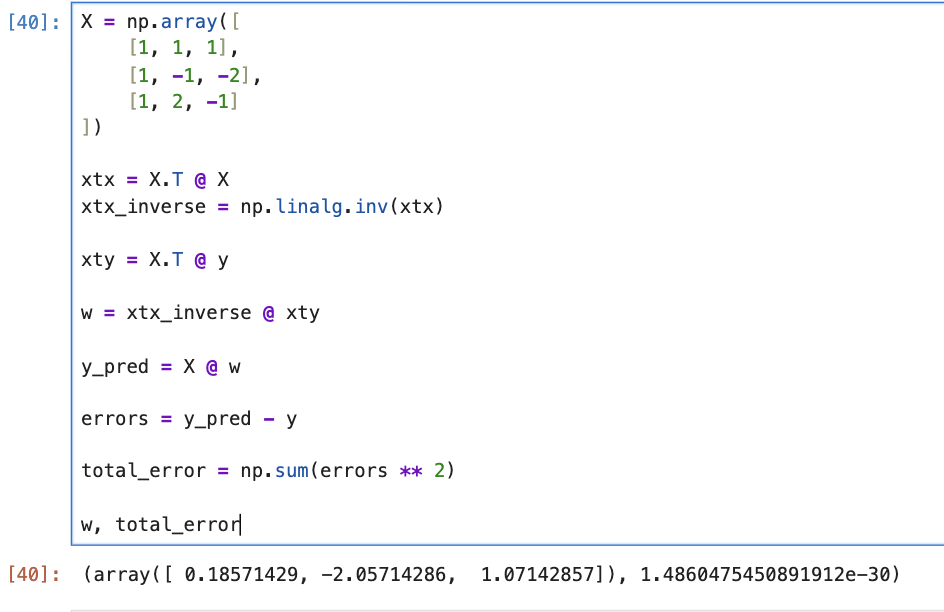
\includegraphics[width=0.5\linewidth]{image1.png}
    \label{fig:placeholder}
\end{figure}
Our corresponding total error is: 1.4860475450891912e-30 (essentially zero).

\section*{Question 2}
$y^{(i)} = x^{(i)} + \epsilon^{(i)}, \epsilon - N(0, 1), x \in R$

\begin{center}
\begin{tabular}{|c|c|c|}
-5 & -6.2 & -5.6 \\
0 & 0.7 & 0.6 \\
1 & 2.5 & 1.2 \\
6 & 6.4 & 7.2 \\
\end{tabular}
\end{center}
Compare a linear model: $\hat{y} = w_1 x$ to a polynomial model: $\hat{y} = w_1 x + w_2 x^2$

\subsection*{Part (a):}
Linear model: Since the data is being generated by $y^{(i)} = x^{(i)} + \epsilon^{(i)}$, where $\epsilon$ is our noise with mean zero $(N (mean = 0, SD = 1) )$, that means that y would on average = x. This is because when we have infinite data, the noise would average out since we would have infinity + and - noise, and our model would find the true fit between x and y. Therefore, our parameter would converge to 1. 
- The true function would be y = x (ignore noise)


Polynomial model: With this model, we can take the logic from the linear model and apply $w_1$ converging to 1. For our $w_2 x^2$, our actual generating function does not have a quadratic equation or number. It is strictly liner, which would converge our second parameter to zero and still apply the same rules for our first parameter $w_1$ which converges to 1.

\subsection*{Part (b):}

X (linear) = 
\begin{tabular}{|c|}
\hline
-5 \\
0 \\
1 \\
6 \\
\hline
\end{tabular}
,
X (poly) = 
\begin{tabular}{|c|c|}
\hline
-5  & 25 \\
0  & 0 \\
1 & 1 \\
6 & 36 \\
\hline
\end{tabular}
,
$y_1$ = 
\begin{tabular}{|c|}
\hline
-6.2 \\
0.7 \\
2.5 \\
6.4 \\
\hline
\end{tabular}
,
$y_2$ = 
\begin{tabular}{|c|}
\hline
-5.6 \\
0.6 \\
1.2 \\
7.2 \\
\hline
\end{tabular}

\begin{figure}[h]
\centering
    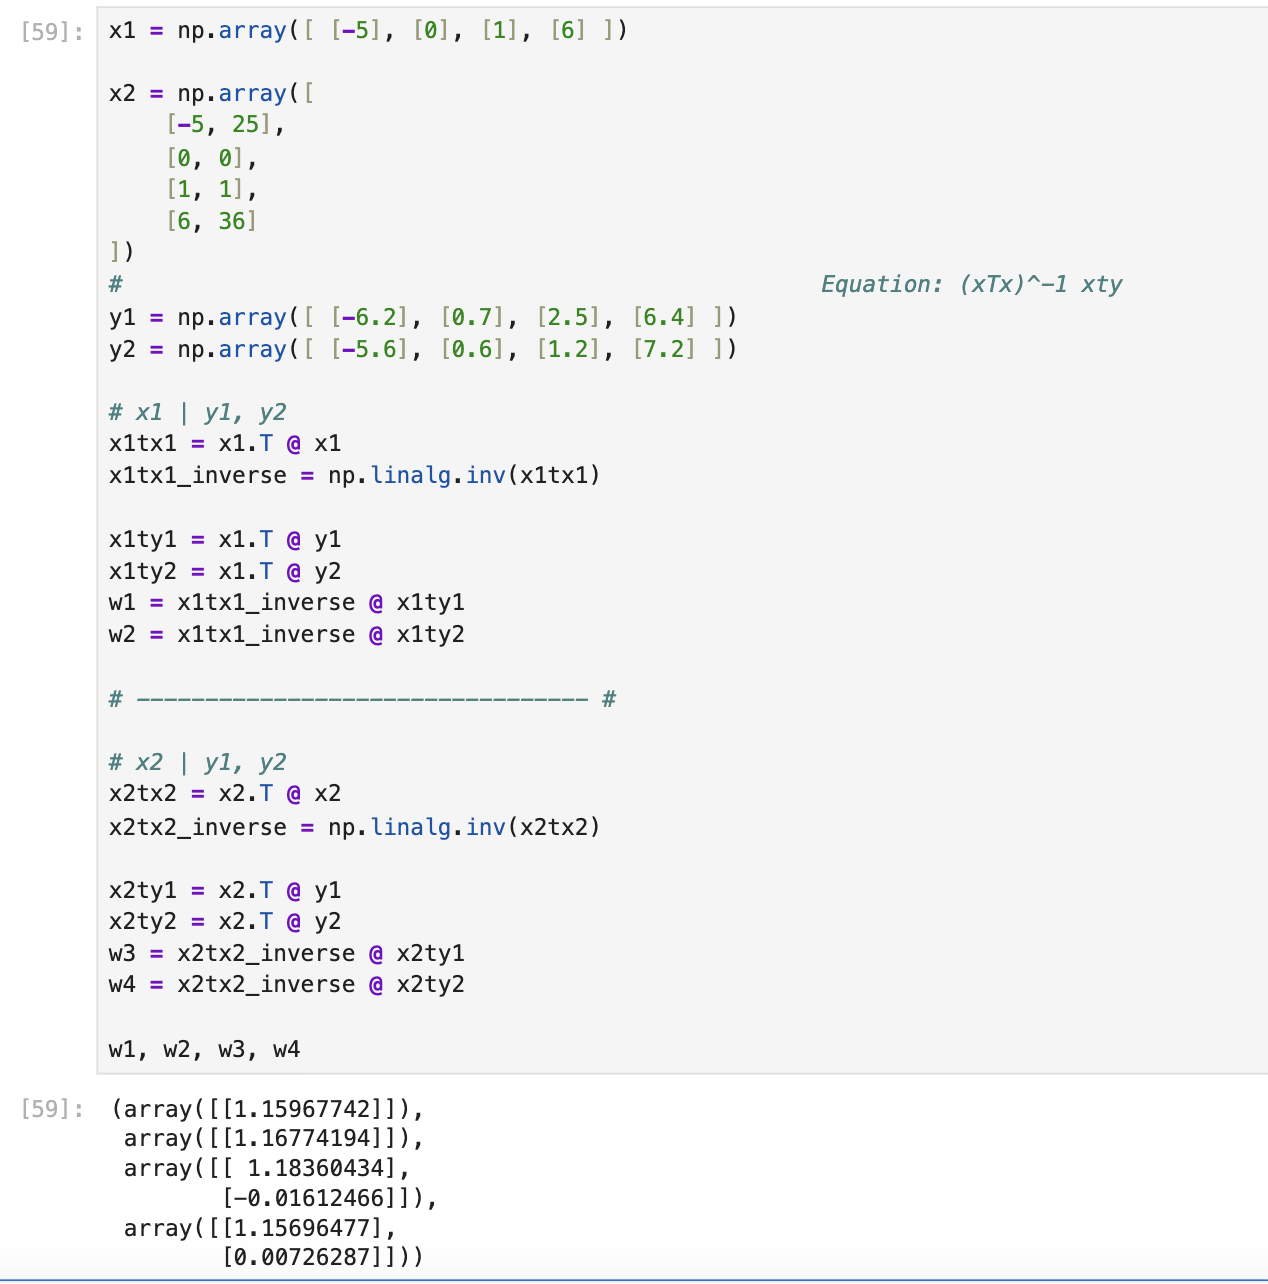
\includegraphics[width=0.5\linewidth]{image3.png}
\end{figure}
With our code above, we get our solutions after using the closed form solution. Our answers become:


- Linear fit for ($x_1, y_1$): 1.159


- Linear fit for ($x_1, y_2$): 1.167


- Polynomial fit for ($x_1, y_1$): [1.183, -0.016]


- Polynomial fit for ($x_1, y_2$): [1.156, 0.007]


\subsection*{Part (c):}


change in $w_1$ for our linear model:

$(x_1, y_2) -(x_1, y_1) = 1.167 - 1.159 = 0.008$

Change in $w_1$ for our polynomial model:

$(x_1, y_2) -(x_1, y_1) = 1.183 - 1.156 = 0.027$


From this, we can see that our polynomial model had a larger change in $w_1$. This is because we have an extra parameter on our polynomial model, which means that small changes in our data lead to larger shifts in our parameters. Both parameters adjust to one another with shifting and fitting the data, which can lead to larger changes. The linear model on the other hand, is what it says; linear, which makes it less flexible and more stable. 


\section*{Question 3}

$x(i) \in R$
,
\begin{tabular}{|c|c|c|}
\hline
1 & 1 & 1 \\
2 & -1 & 0 \\
-3 & -1 & 1 \\
-3 & 1 & 1 \\
\hline
\end{tabular}

\subsection*{Part (a):}

We can use the sigmoid function to simplify our Probability equation (from lecture slides).

$o(z) = \frac{1}{1+e^{-z}}$ where $z = w * x$


- log and e cancel each other out, log($e^x$) = $x_{(i)}$



\[
P(y^{(i)} = +1 | x^{(i)};w) = \frac{1}{1+e^{-z}}
\]
\[
P(y^{(i)} = 0 | x^{(i)};w) = 1 - \frac{1}{1+e^{-z}}
\]

for $z = w_{(i)}*x_{(i)}$: 
\[
\frac{\partial ll(w)}{\partial w_1} = \frac{1}{n}\sum_{i =1}^{n}[y^{(i)} - o(z) * x_1] 
\]
\[
\frac{\partial ll(w)}{\partial w_2} = \frac{1}{n}\sum_{i =1}^{n}[y^{(i)} - o(z) * x_2] 
\]

\subsection*{Part (b):}

\begin{figure}[ht]
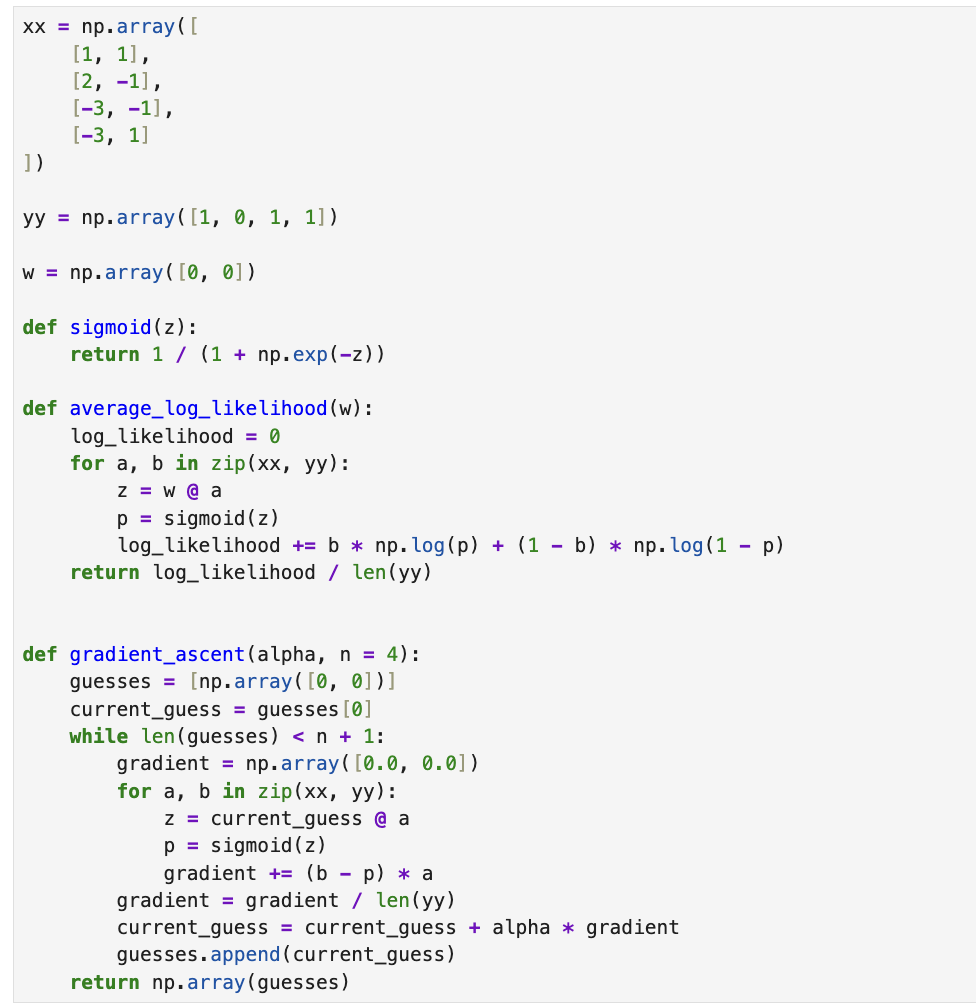
\includegraphics[width=0.4\linewidth]{image5.png}
\end{figure}

\begin{figure}[ht]
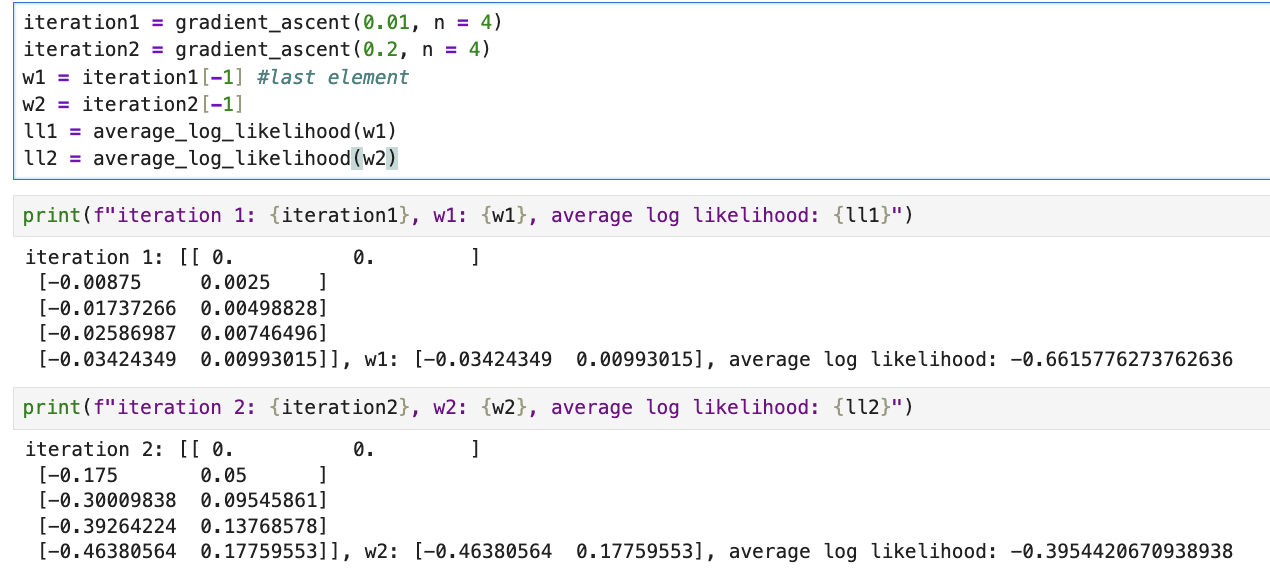
\includegraphics[width=0.7\linewidth]{image6.png}
\end{figure}


\subsection*{Part (c):}

After running 4 iterations with the code given above, the learning rate of alpha = 0.2 is larger than the learning rate of alpha = 0.01. To be more specific, our 0.01 alpha has a smaller average log likelihood of -0.66 compared to our 0.2 alpha which has an average log likelihood of -0.39. This means that the larger learning rate converges more quickly giving us a better and faster solution. 
\end{document}


